\documentclass[10pt,a4paper]{article}
\usepackage{tabularray}
\usepackage{tikz}             
\usepackage{xeCJK}
\usepackage{amsthm}  
\usepackage[fontset=macnew]{ctex}
\usepackage{sgame}
\usepackage{geometry}
\usepackage{amsmath}
\usepackage{amssymb}
\usepackage{graphicx}
\usepackage{sectsty}
\usepackage{color}
\geometry{left=2.cm,right=2.cm,top=3.18cm,bottom=3.18cm}
\usepackage{pgfplots} % package used to implement the plot
\usepackage{pgf-pie}
\usepackage{exscale}
\usepackage{relsize}
\pgfplotsset{width=6.5cm, compat=1.6}
\usepackage{indentfirst}
\usepackage{float}
\usetikzlibrary{shapes,arrows}
\sectionfont{\color{blue}\selectfont}
\subsectionfont{\color{blue}\selectfont}
\subsubsectionfont{\color{blue}\selectfont}
\usepackage{hyperref}
\usepackage{marvosym}
\usepackage{color}
\usepackage{minted}
\usemintedstyle{xcode}
\usepackage{memorygraphs}
\usetikzlibrary{calc,shapes.multipart,chains,arrows.meta}
\usepackage{caption}
\usepackage{makecell}
\newtheorem{definition}{定义}
\newtheorem{theorem}{\textcolor{red}{定理}}
\newtheorem*{solution}{\kaishu 解}
\usepackage[skins]{tcolorbox} %必须标注skin,才能使用shadow命令显示阴影。
\tcbuselibrary{breakable} %breakable:支持跨页
\usepackage{fancyhdr} % 导入fancyhdr包
\pagestyle{fancy}
% 页眉设置
\fancyhead[L]{\textbf{龚舒凯\ 2022202790}}

\begin{document}
	\title{{\Huge 数据结构与算法I实验报告{\large\linebreak\\}}{\huge 实验1:栈和队列的应用\linebreak\linebreak}}
	\vspace{3cm}
	%\author{\Large 龚舒凯\ 2022202790\ 应用经济-数据科学实验班}
	\author{\\ \Large 龚舒凯\ 2022202790\ 应用经济-数据科学实验班\\
		\hfill\\
		\Large{\url{https://github.com/GONGSHUKAI}}\\
		\hfill}
	
	\date{\today}
	\maketitle
	\newpage
	\begin{center}
		{\huge \textbf{骑士巡逻}}
	\end{center}
	\section{需求分析}
	\noindent \textbf{问题描述:}骑士巡逻(Knight's tour)是指在按照国际象棋中骑士的规定走法走遍整个棋盘的每一个方格,而且每个网格只能够经过一次。假若骑士能够走回到最初位置,则称此巡逻为“封闭巡逻”,否则,称为“开巡逻”。\\
	国际象棋中骑士的走法与中国象棋中马的走法相似,呈“日”字型或“L”字型。如下图所示。即每走一步,其行列坐标,一个变化1,另一个变化2。
	\begin{figure}[htbp]
		\centering
		\begin{minipage}{0.49\linewidth}
			\centering
			\includegraphics[width=0.5\linewidth]{Knight's Tour}
			\caption{骑士可走的8个方向}
		\end{minipage}
		\begin{minipage}{0.49\linewidth}
			\centering
			\includegraphics[width=0.5\linewidth]{Result}
			\caption{一种“开巡逻”}
		\end{minipage}		
	\end{figure}
	
	\noindent \textbf{基本要求:}将骑士放在给定大小($n\times n$)的国际象棋棋盘的给定位置上(某一方格中),骑士按照走棋规则进行移动,要求每个方格只进入一次,走遍棋盘上的所有方格。分别编写\textbf{一个递归和一个非递归程序},求出骑士的行走路线,将数字1,2,3,...,$n\times n$依次填入这个棋盘上的所有方格,数字表示路线上的第几步。\\
	
	\noindent \textbf{输入形式:}棋盘的大小$n$(只考虑正方形的棋盘,即棋盘上共有$n\times n$个方格);骑士在棋盘上的起始位置$(x, y)$。\\
	
	\noindent \textbf{输出形式:}骑士完成一次巡逻的路线(即每个方格标注了从$1$到$n\times n$不同数字的棋盘)。例如,对于一个$5\times 5$的棋盘,若骑士从$(2,2)$开始巡逻,则一种巡逻路线可以为:\\
	\begin{center}
		$\begin{bmatrix}
		21&2&7&12&23\\
		8&13&22&17&6\\
		3&20&1&24&11\\
		14&9&18&5&16\\
		19&4&15&10&25
		\end{bmatrix}$
	\end{center}
	\newpage
	\section{概要设计}
	\noindent \textbf{1.递归程序:}考虑使用深度优先搜索遍历(DFS)实现。设置目标搜索深度为$n\times n$(棋盘格数),从起始位置开始,向骑士能走的8个方向搜索,如果搜索失败就回溯。当搜索深度达到$n^2$时输出棋盘巡逻结果。\\

	\noindent \textbf{2.非递归程序:}考虑使用栈实现。设置目标搜索深度为$n\times n$(棋盘格数),从起始位置开始,向骑士能走的8个方向搜索,将每次骑士走的坐标入栈,如果搜索失败就将栈顶坐标弹出。当搜索深度达到$n^2$时输出栈中每一个坐标。
	\subsection{抽象数据类型} 
	\noindent 在本程序中,用到的\textbf{抽象数据类型}定义如下所示:\\
	
	\noindent ADT \mintinline{C}|coord|$\{$
	
	数据对象:$D=\{c | c\in \mintinline{C}|int|\}$
	
	数据关系:$R=\{ \left\langle e_1,e_2\right\rangle | e_1,e_2 \in \mintinline{C}|int|,e_1\text{表示骑士所在行},e_2\text{表示骑士所在列}\}$
	
	基本操作:
	
	\qquad \mintinline{C}|Position(row, col)| 操作结果:返回一个\mintinline{C}|coord|类型的坐标\mintinline{C}|(row,col)|
	
	\noindent $\}$
	
	\noindent ADT \mintinline{C}|stack|$\{$
	
	数据对象:$D=\{c | c\in \mintinline{C}|int|\}$
	
	数据关系:$R=\{ \left\langle e_1,e_2\right\rangle | e_1\text{是一个}\mintinline{C}|int[]|\text{类型的数组,}e_2\text{是一个指向栈顶的指针}\}$
	
	基本操作:
	
	\qquad \mintinline{C}|InitStack()| 操作结果:创建一个字符串类型的栈
	
	\qquad \mintinline{C}|StackPush(s, value)| 操作结果:入栈骑士的坐标
	
	\qquad \mintinline{C}|StackPop(s)| 操作结果:将栈顶元素弹出
	
	\qquad \mintinline{C}|PrintStack(s, ChessBoard[N][N], n, sum)|
	
	\qquad 操作结果:打印栈中储存的骑士巡逻坐标,$n$为棋盘格大小,\mintinline{C}|sum|为骑士巡逻的方法数。
	
	\noindent $\}$
	\subsection{主程序流程}
	\noindent
	\begin{enumerate}
		\item 创建棋盘\mintinline{C}|ChessBoard[N][N]|并将所有元素置0,创建一个储存骑士坐标的栈\mintinline{C}|patrol|。
		\item 输入棋盘的边长和骑士巡逻的初始位置。
		\item 调用\mintinline{C}|KnightPatrol_Recursion(ChessBoard, row, col, n)|和\\
		\mintinline{C}|KnightPatrol_Stack(ChessBoard, row, col, n, patrol)|,输出骑士巡逻的所有可能路线。
	\end{enumerate}
	\newpage
	\section{详细设计}
	\noindent 坐标\mintinline{C}|coord|和栈\mintinline{C}|stack|的基本操作设计在附录中有详细代码实现。这里主要阐述\textbf{两种骑士巡逻实现函数(递归回溯实现和栈实现)的详细设计。}
	\subsection{递归回溯法实现骑士巡逻路线}
	\noindent 递归回溯法寻找骑士巡逻路线的函数定义如下:
	\begin{center}
		\mintinline{C}|void KnightPatrol_Recursion(int ChessBoard[N][N], int row, int col, int n);|
	\end{center}
	其中\mintinline{C}|ChessBoard[N][N]|为大棋盘,\mintinline{C}|row|为骑士所在行,\mintinline{C}|col|为骑士所在列,\mintinline{C}|n|为棋盘边长。设\mintinline{C}|N|为全局变量,表示棋盘边长的上限。\\

	\noindent \textbf{算法设计如下:由于骑士最终必然要遍历完$n^2$个棋盘格,因此设置最大搜索深度为\mintinline{C}|depth = n * n|}
	\begin{enumerate}
		\item 如果到达了最大搜索深度:
		\begin{enumerate}
			\item 当搜索到一种巡逻路线时,首先将这个巡逻路线打印出来。
			\item 然后递归回溯,寻找其他的巡逻路线。
		\end{enumerate}
		\item 如果没有到达最大搜索深度:向八个方向移动骑士,如果移动位置合法:
		\begin{enumerate}
			\item 标记骑士巡逻过这个棋盘格,并递归搜索。
			\item 如果深度优先搜索一直没搜到解,则将搜索过的棋盘格置0,并递归回溯,表示从这一步搜索退回来。
		\end{enumerate}
	\end{enumerate}
	代码实现如下:
	\begin{minted}[mathescape,linenos,numbersep=5pt,gobble=2,frame=lines,framesep=2mm]{C++}
		void KnightPatrol_Recursion(int ChessBoard[N][N], int row, int col, int n){
			//递归回溯法解决骑士巡逻问题
			//row, col是骑士的行列
			if (depth >= n * n){ //搜索深度达到n*n说明已经搜到答案
				sum++;//骑士巡逻方法数+1
				PrintChessboard(ChessBoard, n, sum);
				flag = 1;//骑士巡逻路线存在
				return;//回溯
			}
			for (int i = 0 ; i < 8 ; i++){//骑士分别向8个方向移动
				int new_row = row + step[i][0];
				int new_col = col + step[i][1];
				//如果移动方向合法,且该方向之前没有走过
				if (ValidIndex(new_row, new_col, n) == true && ChessBoard[new_row][new_col] == 0){
					ChessBoard[new_row][new_col] = ++depth;
					KnightPatrol_Recursion(ChessBoard, new_row, new_col, n);//从新位置开始搜索
					//到这里仍然没搜到,则说明这条路走不通,需回溯
					depth--;//搜索深度-1
					ChessBoard[new_row][new_col] = 0;//搜索过的位置置零
				}
			}
		}
	\end{minted}
	\subsection{依托栈的非递归法寻找骑士巡逻路线}
	\noindent 依托栈的非递归法寻找骑士巡逻路线的函数定义如下:
	\begin{center}
		\mintinline{C}|void KnightPatrol_Stack(int ChessBoard[N][N], int row, int col, int n, stack *patrol);|
	\end{center}
	其中\mintinline{C}|ChessBoard[N][N]|为大棋盘,\mintinline{C}|row|为骑士所在行,\mintinline{C}|col|为骑士所在列,\mintinline{C}|n|为棋盘边长,\mintinline{C}|patrol|为储存骑士移动位置的栈。设\mintinline{C}|N|为全局变量,表示棋盘边长的上限。\\

	\noindent \textbf{算法设计如下:由于骑士最终必然要遍历完$n^2$个棋盘格,因此设置最大搜索深度为\mintinline{C}|depth = n * n|}
	\begin{enumerate}
		\item 如果到达了最大搜索深度:
		\begin{enumerate}
			\item 当搜索到一种巡逻路线时,首先将这个巡逻路线打印出来。
			\item 然后递归回溯,寻找其他的巡逻路线。
		\end{enumerate}
		\item 如果没有到达最大搜索深度:向八个方向移动骑士,如果移动位置合法:
		\begin{enumerate}
			\item 标记骑士巡逻过这个棋盘格,并将当前位置入栈,从这个位置开始下一步的巡逻。
			\item 如果深度优先搜索一直没搜到解,则将搜索深度减1,把栈顶元素弹出,表示从这一步搜索退回来。
		\end{enumerate}
	\end{enumerate}
	代码实现如下:
	\begin{minted}[mathescape,linenos,numbersep=5pt,gobble=2,frame=lines,framesep=2mm]{C++}
		void KnightPatrol_Stack(int ChessBoard[N][N], int row, int col, int n, stack *patrol){
			//非递归法解决骑士巡逻问题
			//row, col是骑士的行列
			if (depth2 == n * n){ //搜索深度达到n*n说明已经搜到答案
				sum2++;//骑士巡逻方法数+1
				PrintStack(patrol, ChessBoard, n, sum2);
				flag2 = 1;//骑士巡逻路线存在
				return;//回溯
			}
			for (int i = 0 ; i < 8 ; i++){//骑士分别向8个方向移动
				int new_row = row + step[i][0];
				int new_col = col + step[i][1];
				//如果移动方向合法,且该方向之前没有走过
				if (ValidIndex(new_row, new_col, n) == true && ChessBoard[new_row][new_col] == 0){
					ChessBoard[new_row][new_col] = ++depth2;
					coord *nextpos = Position(new_row, new_col);//记录新位置
					StackPush(patrol, *nextpos);//将新位置入栈
					KnightPatrol_Stack(ChessBoard, new_row, new_col, n, patrol);//从新位置开始搜索
					//到这里仍然没搜到,则说明这条路走不通,需回溯
					ChessBoard[new_row][new_col] = 0;//搜索过的位置置零
					depth2--;//搜索深度-1
					StackPop(patrol);//将走不通的位置弹出栈
				}
			}
		}
	\end{minted}
	\newpage
	\section{用户使用说明}
	\noindent 1.程序运行后,首先显示"请输入棋盘的边长$n$:"
	\begin{itemize}
		\item 输入一个正整数$n$:$n$的范围为\mintinline{C}|3 <= n <= 8|,骑士的走法决定其无法在边长$<3$的棋盘中巡逻。当$n>8$时,递归回溯法的运算时间过长。
	\end{itemize}
	\noindent 2.其次显示"请输入骑士在棋盘上的起始位置\mintinline{C}|row, col|:"
	\begin{itemize}
		\item 输入两个正整数\mintinline{C}|row, col|:\mintinline{C}|row, col|的范围为\mintinline{C}|0 <= row, col <= n|。
		\item 两个正整数以空格分割。一个合法的输入为\mintinline{C}|0, 0|
		\item \mintinline{C}|0,0|、\mintinline{C}|00|等等都是不合法的输入。
	\end{itemize}
	\subsection{测试结果}
	\noindent 有以下测试样例供参考:
	\begin{align*}
		\text{第一组:输入:}&\mintinline{C}|5|\\
		&\mintinline{C}|2 2|\\
		\\
		\text{第二组:输入:}&\mintinline{C}|8|\\
		&\mintinline{C}|0 0|
	\end{align*}
	以第一组测试结果为例:
	\begin{minted}[mathescape,linenos,numbersep=5pt,gobble=2,frame=lines,framesep=2mm]{C++}
			骑士巡逻方法1:递归回溯法:
			骑士巡逻路线1
			23 10 15 4 25 
			16 5 24 9 14 
			11 22 1 18 3 
			6 17 20 13 8 
			21 12 7 2 19 

			...(省略63个骑士巡逻路线结果)

			骑士巡逻方法2:依托栈实现的非递归法:
			骑士巡逻路线1
			23 10 15 4 25 
			16 5 24 9 14 
			11 22 1 18 3 
			6 17 20 13 8 
			21 12 7 2 19 

			...(省略63个骑士巡逻路线结果)
	\end{minted}
	\newpage
	\section{调试分析}
	\subsection{算法的时空分析}
	\subsubsection{递归程序}
	\noindent \textbf{1.时间复杂度:}

		我们可以将递归搜索的过程看作树的遍历:我们将每个坐标视作树的结点,由于骑士可以往8个方向移动,因此初始结点\mintinline{C}|(x,y)|的子节点最多有8个,每个子节点又有8个子节点,以此类推...由于搜索深度为$n^2$(棋盘格数),因此树的最大深度为$n^2$。
		\begin{center}
			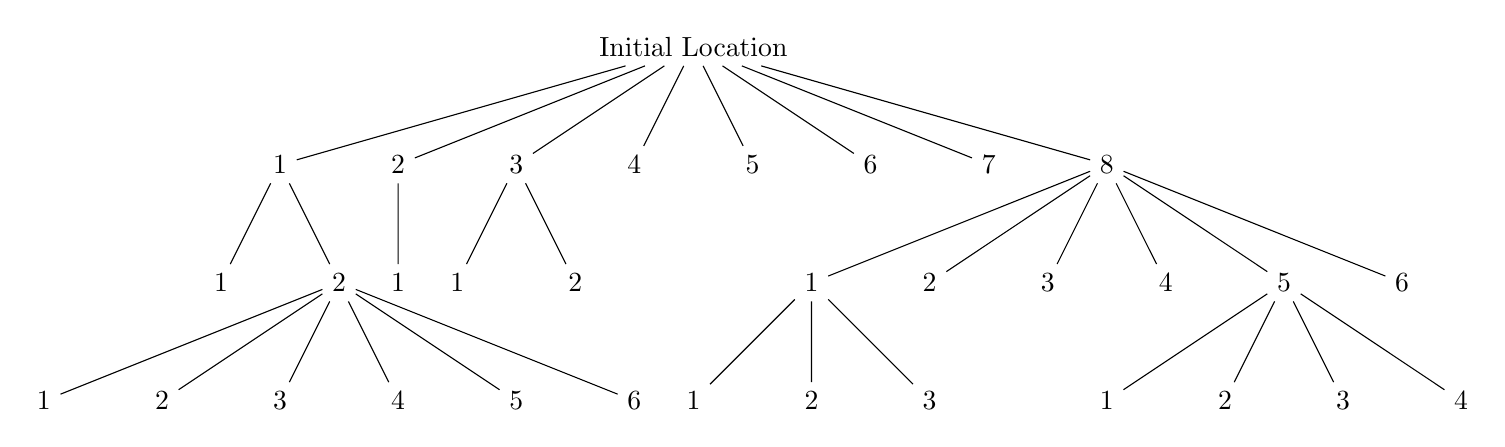
\begin{tikzpicture}
				\node {Initial Location}
					child {
						node{1}
						child {node {1}}
						child {
							node {2}
							child {node {1}}
							child {node {2}}
							child {node {3}}
							child {node {4}}
							child {node {5}}
							child {node {6}}
						}
					}
					child {
						node {2}
						child {node {1}}
					}
					child {
						node {3}
						child {node {1}}
						child {node {2}}
					}
					child {node {4}}
					child {node {5}}
					child {node {6}}
					child {node {7}}
					child {
						node {8}
						child {
							node {1}
							child {node {1}}
							child {node {2}}
							child {node {3}}
						}
						child {node {2}}
						child {node {3}}
						child {node {4}}
						child {
							node {5}
							child {node {1}}
							child {node {2}}
							child {node {3}}
							child {node {4}}
						}
						child {node {6}}
					}
				;
			\end{tikzpicture}
		\end{center}

		尽管不是每个节点都有8个子节点(有一些位置下标越界或已经被访问过),但我们可以计算一个上界,即这个算法最坏情况下会生成$8^{n^2}$个状态空间,时间复杂度$O(8^{n^2})=O(2^n)$,是指数级别的。
		
		棋盘的边长为算法运行时间的主要影响因素,当$n>5$时,算法的计算时间显著变长甚至不可计算(例如棋盘边长$n=6$,初始巡逻位置$(0,0)$时,共有524486种巡逻路线,耗时991.126秒)。
		
		此外,骑士的初始位置队算法的运行时间也有影响。当$n=5$,初始位置为$(0,0)$的骑士巡逻路线共有304条,而当$n=5$,初始位置为$(2,2)$的骑士巡逻路线共有64条,显然初始位置在$(0,0)$的计算时间更长。\\

	\noindent \textbf{2.空间复杂度:}
	
	如果我们用树的观点看待递归回溯法求解骑士巡逻问题的话,该算法占用结点数的上界为$8^{n^2}$。因此算法的最坏空间复杂度为$O(8^{n^2})=O(2^n)$。

	\subsubsection{非递归程序}
	\noindent \textbf{1.时间复杂度:}
	
	类似地,从初始点开始搜索骑士巡逻路径,有最多8个方向可以走,选择一个方向后把这个位置压入栈,又有最多8个方向可以走...以此类推,骑士共需要尝试$n^2$个位置,从而时间复杂度为$O(8^{n^2})=O(2^n)$。\\

	\noindent \textbf{2.空间复杂度:}

	由于我们用栈保存骑士每次巡逻的坐标,用一个数组\mintinline{C}|ChessBoard[N][N]|保存骑士的巡逻顺序,因此算法的空间复杂度为$O(N^2)$,其中$N$为棋盘的最大边长。
	\newpage
	\section{附录}
	\noindent 详细的代码实现如下所示。也可以通过\url{https://github.com/GONGSHUKAI/Data_Structure/tree/main/Lab_Code/Lab_1/Sept.29_Lab}下载代码原文件。
	\begin{minted}[mathescape,gobble=2,frame=lines,framesep=2mm]{C++}
		#include <iostream>
		#include <ctime>
		#define N 8 
		#define MAXSIZE 1000

		using namespace std;

		//骑士的8个移动方向用step[][]记录
		//第一个分量表示行位移,第二个分量表示列位移
		int step[8][2]={{2,1},{1,2},{-1,2},{-2,1},{-2,-1},{-1,-2},{1,-2},{2,-1}};
		int depth = 0;//搜索深度,最大为n*n(棋盘格大小)
		int depth2 = 0;//搜索深度,最大为n*n(棋盘格大小)
		int sum = 0;//记录骑士巡逻的方法数(回溯法)
		int sum2 = 0;//记录骑士巡逻的方法数(非递归法)
		int flag = 0;//判断骑士巡逻路线是否存在(回溯法)
		int flag2 = 0;//判断骑士巡逻路线是否存在(非递归法)

		typedef struct coord{
			int row;
			int col;
		}coord;//存放骑士的位置(row, col)

		typedef struct stack{
			coord data[MAXSIZE];
			int top;
		}stack;//存放骑士位置的栈

		stack* InitStack();//初始化栈
		bool StackEmpty(stack *s);//判断栈空
		coord StackTop(stack *s);//判断栈满
		void StackPush(stack *s, coord value);//入栈骑士的位置(row, col)
		void StackPop(stack *s);//弹出栈顶元素
		//打印栈中储存的骑士巡逻坐标,n为棋盘格大小,sum为骑士巡逻的方法数
		void PrintStack(stack *s, int ChessBoard[N][N], int n, int sum);

		coord* Position(int row, int col);//输入骑士所在行列,返回骑士所在坐标
		bool ValidIndex(int i, int j,int n);//判断[i][j]是否为一个合法的位置
		//打印整个棋盘,n为棋盘格大小,sum为骑士巡逻的方法数
		void PrintChessboard(int ChessBoard[N][N], int n, int sum);
		//递归回溯法寻找骑士巡逻路线
		void KnightPatrol_Recursion(int ChessBoard[N][N], int row, int col, int n);
		//依托栈的非递归法寻找骑士巡逻路线
		void KnightPatrol_Stack(int ChessBoard[N][N], int rol, int col, int n, stack *patrol);

		int main(){
			int ChessBoard[N][N];
			int n;//棋盘大小
			int row, col;//骑士的起始位置
			memset(ChessBoard, 0, sizeof(ChessBoard));//将棋盘置0
			
			cout << "请输入棋盘的边长n:";
			cin >> n;
			cout << "请输入骑士在棋盘上的起始位置row, col:";
			cin >> row >> col;
			
			cout << "骑士巡逻方法1:递归回溯法:" << endl;
			clock_t startTime = clock();//计时开始
			ChessBoard[row][col] = ++depth;
			KnightPatrol_Recursion(ChessBoard, row, col, n);
			if (flag == 0) cout << "不存在骑士巡逻路线" << endl;
			clock_t endTime = clock();//计时结束
			cout << "运行时间:" <<(double)(endTime - startTime) / CLOCKS_PER_SEC << "s" << endl;
			
			memset(ChessBoard, 0, sizeof(ChessBoard));//将棋盘置0
			cout << "骑士巡逻方法2:依托栈实现的非递归法:" << endl;
			clock_t startTime2 = clock();//计时开始
			stack *patrol = InitStack();//创建一个存放骑士坐标的栈
			coord *init = Position(row, col);//骑士的初始位置
			StackPush(patrol, *init);
			ChessBoard[row][col] = ++depth2;
			KnightPatrol_Stack(ChessBoard, row, col, n, patrol);
			if (flag2 == 0) cout << "不存在骑士巡逻路线" << endl;
			clock_t endTime2 = clock();//计时结束
			cout << "运行时间:" <<(double)(endTime2 - startTime2) / CLOCKS_PER_SEC << "s" << endl;
			
		}

		stack* InitStack(){
			stack *s = new stack;
			s->top = -1;//栈顶指针(即数组下标)赋初值-1
			return s;
		}

		bool StackEmpty(stack *s){//如果栈空返回1,否则返回0
			if (s->top == -1) return true;
			else return false;
		}

		coord StackTop(stack *s){//返回栈顶元素
			if (s->top > -1 && s->top < MAXSIZE) return s->data[s->top];
			else{
				coord wrongpos;
				wrongpos.row = -1;
				wrongpos.col = -1;
				return wrongpos;
			}
		}

		void StackPush(stack *s, coord value){//压入栈
			if (s->top == MAXSIZE - 1) return;
			else s->data[++s->top] = value;
		}

		void StackPop(stack *s){//弹出栈顶元素
			if (s->top == -1) return;
			else{
				s->top--;
			}
		}

		coord* Position(int row, int col){
			coord *pos = new coord;
			pos->row = row;
			pos->col = col;
			return pos;
		}

		bool ValidIndex(int i, int j,int n){//n是棋盘的大小
			if (i >= 0 && j >= 0 && i < n && j < n) return true;
			else return false;
		}

		void PrintChessboard(int ChessBoard[N][N], int n, int sum){
			cout << "骑士巡逻路线" << sum << endl;
			for (int i = 0 ; i < n ; i++){
				for (int j = 0 ; j < n ; j++){
					cout << ChessBoard[i][j] << " ";
				}
				cout << endl;
			}
			cout << endl;
		}

		void PrintStack(stack *s, int ChessBoard[N][N], int n, int sum){
			for (int i = 0 ; i <= s->top ; i++){
				ChessBoard[s->data[i].row][s->data[i].col] = i+1;
			}
			PrintChessboard(ChessBoard, n, sum);
		}

		void KnightPatrol_Recursion(int ChessBoard[N][N], int row, int col, int n){
			//递归回溯法解决骑士巡逻问题
			//row, col是骑士的行列
			if (depth >= n * n){ //搜索深度达到n*n说明已经搜到答案
				sum++;//骑士巡逻方法数+1
				PrintChessboard(ChessBoard, n, sum);
				flag = 1;//骑士巡逻路线存在
				return;//回溯
			}
			for (int i = 0 ; i < 8 ; i++){//骑士分别向8个方向移动
				int new_row = row + step[i][0];
				int new_col = col + step[i][1];
				//如果移动方向合法,且该方向之前没有走过
				if (ValidIndex(new_row, new_col, n) == true && ChessBoard[new_row][new_col] == 0){
					ChessBoard[new_row][new_col] = ++depth;
					KnightPatrol_Recursion(ChessBoard, new_row, new_col, n);//从新位置开始搜索
					//到这里仍然没搜到,则说明这条路走不通,需回溯
					depth--;//搜索深度-1
					ChessBoard[new_row][new_col] = 0;//搜索过的位置置零
				}
			}
		}

		void KnightPatrol_Stack(int ChessBoard[N][N], int row, int col, int n, stack *patrol){
			//非递归法解决骑士巡逻问题
			//rol, col是骑士的行列
			if (depth2 == n * n){ //搜索深度达到n*n说明已经搜到答案
				sum2++;//骑士巡逻方法数+1
				PrintStack(patrol, ChessBoard, n, sum2);
				flag2 = 1;//骑士巡逻路线存在
				return;//回溯
			}
			for (int i = 0 ; i < 8 ; i++){//骑士分别向8个方向移动
				int new_row = row + step[i][0];
				int new_col = col + step[i][1];
				//如果移动方向合法,且该方向之前没有走过
				if (ValidIndex(new_row, new_col, n) == true && ChessBoard[new_row][new_col] == 0){
					ChessBoard[new_row][new_col] = ++depth2;
					coord *nextpos = Position(new_row, new_col);//记录新位置
					StackPush(patrol, *nextpos);//将新位置入栈
					KnightPatrol_Stack(ChessBoard, new_row, new_col, n, patrol);//从新位置开始搜索
					//到这里仍然没搜到,则说明这条路走不通,需回溯
					ChessBoard[new_row][new_col] = 0;//搜索过的位置置零
					depth2--;//搜索深度-1
					StackPop(patrol);//将走不通的位置弹出栈
				}
			}
		}
	\end{minted}
\end{document}